\section{Cronograma para Construção da Ontologia na Aplicação}

A aplicação da ontologia no software envolvem algumas mudanças estruturais na arquitetura e
na refatoração de algumas funcionalidades, como uma busca no banco de dados por um acidente por 
exemplo. Desta forma, a equipe técnica definiu a construção da ontologia na aplicação como um projeto
separado, com cronograma próprio, integrado com o cronograma geral do projeto.
O objetivo é encarar a construção como uma mudança de requisitos, estudando o impacto e analisando
as implicações do uso da ontologia dentro da ferramenta, com base nas métricas de qualidade previamente 
definidas. 

\begin{figure}[h]
	\centering
	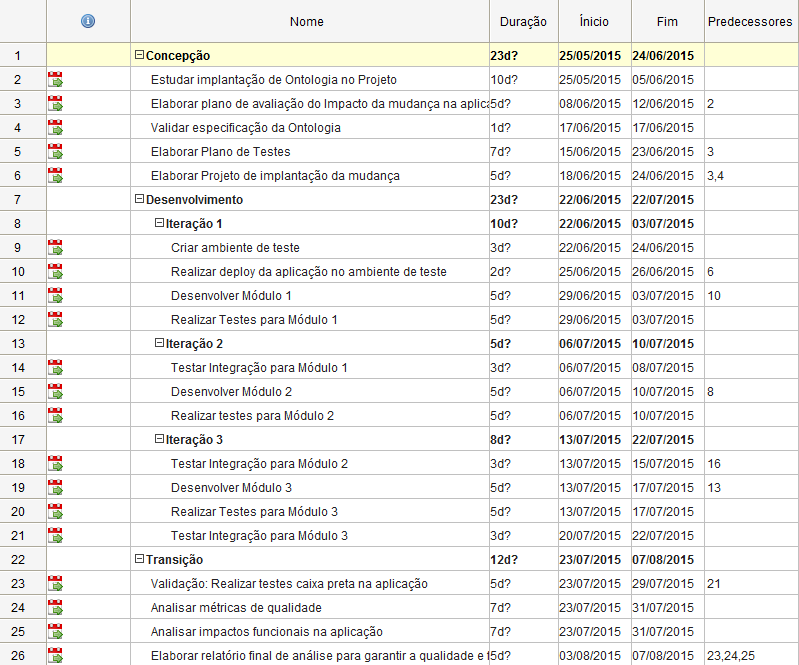
\includegraphics[scale=0.6]{Figuras/cronograma_construcao_ontologia.png}
\end{figure}

\pagebreak

Tabela – Cronograma de Construção da Ontologia na Aplicação

\subsection{Esforço versus Impacto da Construção}

Com base no cronograma, é necessário observar que existe um grau de esforço que será empregado,
com custos inerentes ao processo de software. A mudança mais relevante é o uso do framework \textit{Active RDF} \footnotemark[1], no lugar do \textit{Active Record} que faz deixa transparente o acesso de dados da camada \textit{Model} com o banco de dados. 

A hipótese é de que \textbf{os benefícios da aplicação dessa mudança sejam relevantes a ponto de justificar o custo inerente à mudança do software}. Para analisar a hipótese e refletir sobre suas implicações, foi necessário calcular os custos de produção. O valor considerado pela equipe técnica da hora de um aluno da UnB foi de dez reais e sessenta e cinco centavos, adicionados os valores de consumo de energia e mensalidade da internet. O valor do custo total foi baseado numa rotina de trabalho de 5 horas semanais, durante 58 dias, conforme a divisão de trabalho do cronograma.

O custo total da implementação da mudança na aplicação \textit{Pé na Estrada} ficou em 3088,50 R\$ . Esse valor, divido pelos 58 dias de trabalho, caracterizam 53,25 R\$ por dia de trabalho.

\begin{figure}[h] 
	\centering % para centralizarmos a figura
	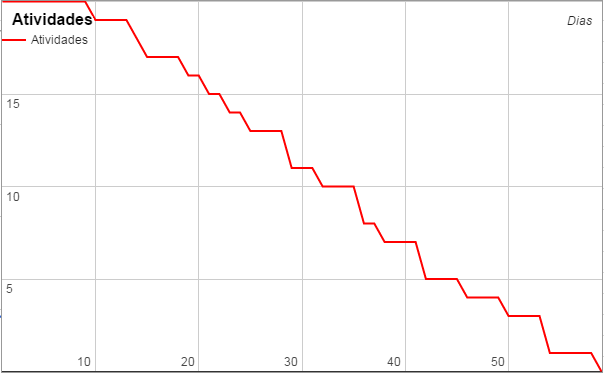
\includegraphics[scale=0.6]{Figuras/grafico_atividades.png} % leia abaixo

\end{figure}

Figura - Burndown das Atividades

\begin{figure}[h] 
	\centering % para centralizarmos a figura
	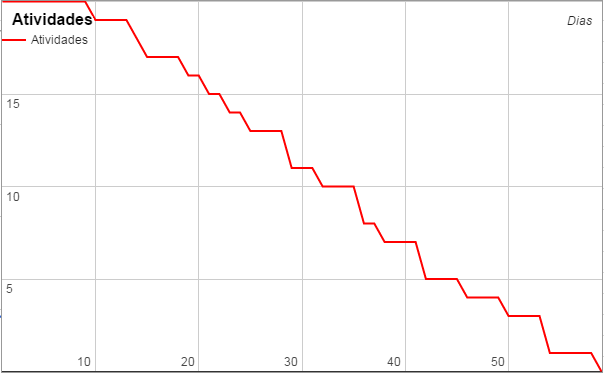
\includegraphics[scale=0.6]{Figuras/grafico_atividades.png} % leia abaixo
	
\end{figure}

Gráfico - Gráfico de Custo Planejado

A discussão sobre os resultados e sobre a hipótese levantada nesse seção serão discutidas no tópico \textbf{Resultados Esperados}. 